
 \documentclass[25pt, a0paper, portrait, margin=0mm, innermargin=15mm,
     blockverticalspace=15mm, colspace=15mm, subcolspace=8mm]{tikzposter} %Default values for poster format options.
     
\usepackage{tabularx,booktabs,adjustbox} % For tables
\usetikzlibrary{calc,fit,arrows,decorations.pathmorphing,backgrounds,fit,positioning}
\usetikzlibrary{shapes.symbols}

% tikz colour settings
\tikzset{pop1/.style={blue!40},pop2/.style={red!40}}

 \tikzposterlatexaffectionproofon %shows small comment on how the poster was made at bottom of poster

 % Commands
 \newcommand{\bs}{\textbackslash}   % backslash
 \newcommand{\cmd}[1]{{\bf \color{red}#1}}   % highlights command

 % Title, Author, Institute
 \title{Efficient simulation of introgression, admixture and local ancestry}
 \author{{\bf Georgia Tsambos}}
 \institute{{\bf University of Melbourne, Australia}}

 % -- PREDEFINED THEMES ---------------------- %
 % Choose LAYOUT:  Default, Basic, Rays, Simple, Envelope, Wave, Board, Autumn, Desert,
 \usetheme{Autumn}
\usecolorstyle[colorPalette=BlueGrayOrange]{Denmark}


 \begin{document}

     \maketitle
   
   %%% BLOCK 0  
 \block[bodyverticalshift=-1cm]{0. Introduction}{
%

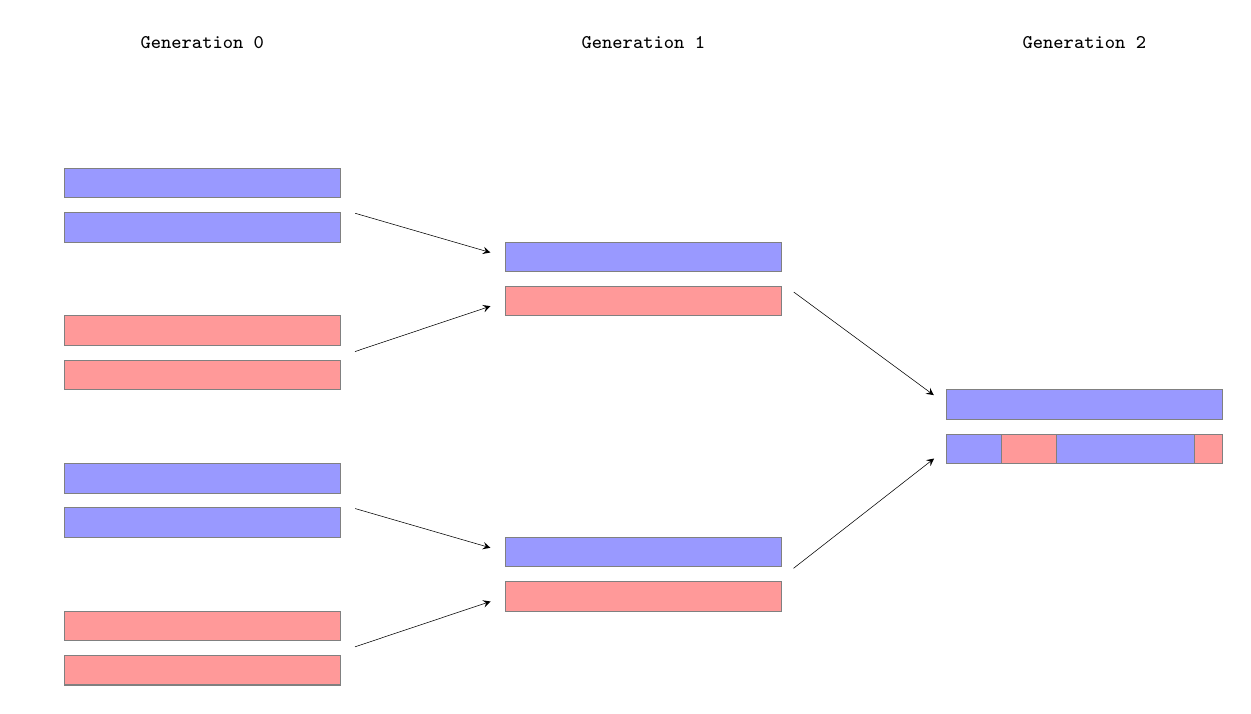
\begin{tikzpicture}[yscale=0.25, xscale=0.35,font=\scriptsize]

\tikzset{
pop1/.style={fill=blue!40,draw=black!50},
pop2/.style={fill=red!40,draw=black!50},
inherit/.style={->,>=stealth,ultra thin,shorten <=2mm,shorten >=2mm,very thin},
recomb/.style={thick,draw=black!70}
}

% Nodes
\node (hapx) at (1,0) {};
\node (hapy) at (0,1.5) {};
\node (hapxy) at ($10*(hapx) + (hapy)$) {};

\node (gen1) at (0,0) {};
\node (gen2) at ($8*(hapx) + 0*(hapx)$) {};
\node (gen3) at ($8*(hapx) + 8*(hapx)$) {};

\node (ind1gen3) at ($(gen3) + (0,0)$) {};
\node (indsep) at ($5*(hapy)$) {};

\node (ind1gen2) at ($(gen2) + 1*(indsep)$) {};
\node (ind2gen2) at ($(gen2) - 1*(indsep)$) {};

\node (ind1gen1) at ($(gen1) + 1.5*(indsep)$) {};
\node (ind2gen1) at ($(gen1) + 0.5*(indsep)$) {};
\node (ind3gen1) at ($(gen1) - 0.5*(indsep)$) {};
\node (ind4gen1) at ($(gen1) - 1.5*(indsep)$) {};

\node (chr1) at ($0.25*(hapy)$)  {};
\node (chr2) at ($-1.25*(hapy)$) {};


% Haplotypes

\filldraw[pop1] ($(gen1) + (ind1gen1) + (chr1)$) rectangle +(hapxy);
\filldraw[pop1] ($(gen1) + (ind1gen1) + (chr2)$) rectangle +(hapxy);

\filldraw[pop2] ($(gen1) + (ind2gen1) + (chr1)$) rectangle +(hapxy);
\filldraw[pop2] ($(gen1) + (ind2gen1) + (chr2)$) rectangle +(hapxy);

\filldraw[pop1] ($(gen1) + (ind3gen1) + (chr1)$) rectangle +(hapxy);
\filldraw[pop1] ($(gen1) + (ind3gen1) + (chr2)$) rectangle +(hapxy);

\filldraw[pop2] ($(gen1) + (ind4gen1) + (chr1)$) rectangle +(hapxy);
\filldraw[pop2] ($(gen1) + (ind4gen1) + (chr2)$) rectangle +(hapxy);


\filldraw[pop1] ($(gen2) + (ind1gen2) + (chr1)$) rectangle +(hapxy);
\filldraw[pop2] ($(gen2) + (ind1gen2) + (chr2)$) rectangle +(hapxy);

\filldraw[pop1] ($(gen2) + (ind2gen2) + (chr1)$) rectangle +(hapxy);
\filldraw[pop2] ($(gen2) + (ind2gen2) + (chr2)$) rectangle +(hapxy);


\filldraw[pop1] ($(gen3) + (ind1gen3) + (chr1)$) rectangle +(hapxy);
\fill[pop1] ($(gen3) + (ind1gen3) + (chr2)$) rectangle +(hapxy);
\fill[pop2] ($(gen3) + (ind1gen3) + (chr2)+ 2*(hapx)$) rectangle ($(gen3) + (ind1gen3) + (chr2)+ (hapxy)$);
\fill[pop1] ($(gen3) + (ind1gen3) + (chr2)+ 4*(hapx)$) rectangle ($(gen3) + (ind1gen3) + (chr2)+ (hapxy)$);
\fill[pop2] ($(gen3) + (ind1gen3) + (chr2)+ 9*(hapx)$) rectangle ($(gen3) + (ind1gen3) + (chr2)+ (hapxy)$);
%\draw ($(gen3) + (ind1gen3) + (chr2)$) rectangle +(hapxy);


% Copying lines

\node (startline) at ($-1*(hapx) + 0.5*(hapy)$) {};
\node (chrdiff) at ($(chr1) - (chr2)$) {};

%\node (hapx) at (1,0) {};

%\draw[recomb] ($(gen1) + (ind1gen1) + (chr1) + (startline)$) -- ++($(hapx)$) --  ++($4*(hapx)$) --  ++($-1*(chrdiff)$) -- ++($2*(hapx)$) -- ++($(chrdiff)$) -- ++($4*(hapx)$) -- ++($1*(hapx)$);
%\draw[recomb] ($(gen1) + (ind2gen1) + (chr2) + (startline)$) -- ++($(hapx)$) -- ++($10*(hapx)$) --  ++($(hapx)$);
%\draw[recomb] ($(gen1) + (ind3gen1) + (chr1) + (startline)$) -- ++($(hapx)$) -- ++($10*(hapx)$) --  ++($(hapx)$);
%\draw[recomb] ($(gen1) + (ind4gen1) + (chr2) + (startline)$) -- ++($(hapx)$) --  ++($5*(hapx)$) --  ++($(chrdiff)$) -- ++($2*(hapx)$) -- ++($3*(hapx)$) -- ++($1*(hapx)$);
%
%\draw[recomb] ($(gen2) + (ind1gen2) + (chr1) + (startline)$) -- ++($(hapx)$) -- ++($10*(hapx)$) --  ++($(hapx)$);
%\draw[recomb] ($(gen2) + (ind2gen2) + (chr1) + (startline)$) -- ++($(hapx)$) --  ++($2*(hapx)$) --  ++($-1*(chrdiff)$) -- ++($2*(hapx)$) -- ++($(chrdiff)$) -- ++($3*(hapx)$) -- ++($2*(hapx)$) -- ++($-1*(chrdiff)$) -- ++($(hapx)$) -- ++($(hapx)$) ;


% Arrows
\draw[inherit] ($(gen1) + (ind1gen1) + (chr2) + 10*(hapx) + 0.75*(chrdiff)$) -- ($(gen2) + (ind1gen2) + (chr1) + 0.5*(hapy)$);
\draw[inherit] ($(gen1) + (ind2gen1) + (chr2) + 10*(hapx) + 0.75*(chrdiff)$) -- ($(gen2) + (ind1gen2) + (chr2) + 0.5*(hapy)$);
\draw[inherit] ($(gen1) + (ind3gen1) + (chr2) + 10*(hapx) + 0.75*(chrdiff)$) -- ($(gen2) + (ind2gen2) + (chr1) + 0.5*(hapy)$);
\draw[inherit] ($(gen1) + (ind4gen1) + (chr2) + 10*(hapx) + 0.75*(chrdiff)$) -- ($(gen2) + (ind2gen2) + (chr2) + 0.5*(hapy)$);

\draw[inherit] ($(gen2) + (ind1gen2) + (chr2) + 10*(hapx) + 0.75*(chrdiff)$) -- ($(gen3) + (ind1gen3) + (chr1) + 0.5*(hapy)$);
\draw[inherit] ($(gen2) + (ind2gen2) + (chr2) + 10*(hapx) + 0.75*(chrdiff)$) -- ($(gen3) + (ind1gen3) + (chr2) + 0.5*(hapy)$);


% Labels
\node (lab1) at ($(gen1) + 2.5*(indsep) + 0.5*(hapxy)$) {$\texttt{Generation 0}$};
\node (lab2) at ($2*(gen2) + 2.5*(indsep) + 0.5*(hapxy)$) {$\texttt{Generation 1}$};
\node (lab3) at ($4*(gen2) + 2.5*(indsep) + 0.5*(hapxy)$) {$\texttt{Generation 2}$};

\end{tikzpicture}
 
%here is some text
 }
 \begin{columns}
 \begin{subcolumns}
   \subcolumn{20} \block[bodyoffsetx=1cm]{}{Some text about my favourite thing }
   \subcolumn{4}  \block{}{ 

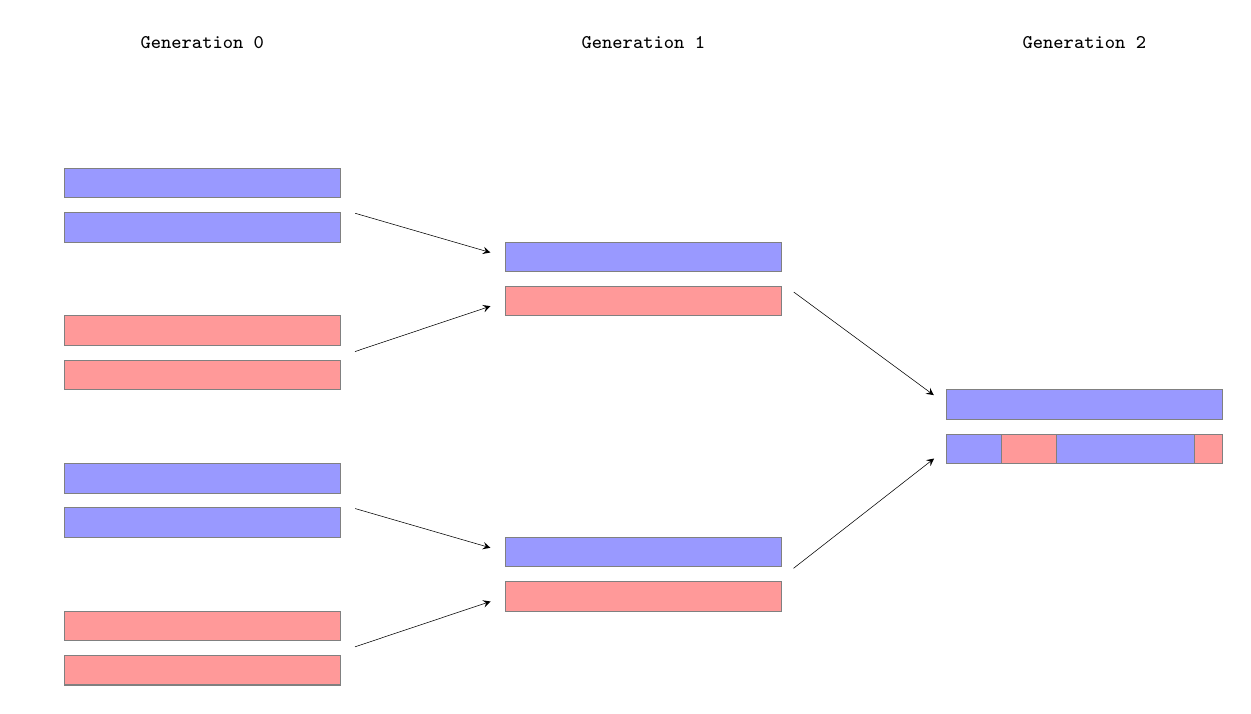
\begin{tikzpicture}[yscale=0.25, xscale=0.35,font=\scriptsize]

\tikzset{
pop1/.style={fill=blue!40,draw=black!50},
pop2/.style={fill=red!40,draw=black!50},
inherit/.style={->,>=stealth,ultra thin,shorten <=2mm,shorten >=2mm,very thin},
recomb/.style={thick,draw=black!70}
}

% Nodes
\node (hapx) at (1,0) {};
\node (hapy) at (0,1.5) {};
\node (hapxy) at ($10*(hapx) + (hapy)$) {};

\node (gen1) at (0,0) {};
\node (gen2) at ($8*(hapx) + 0*(hapx)$) {};
\node (gen3) at ($8*(hapx) + 8*(hapx)$) {};

\node (ind1gen3) at ($(gen3) + (0,0)$) {};
\node (indsep) at ($5*(hapy)$) {};

\node (ind1gen2) at ($(gen2) + 1*(indsep)$) {};
\node (ind2gen2) at ($(gen2) - 1*(indsep)$) {};

\node (ind1gen1) at ($(gen1) + 1.5*(indsep)$) {};
\node (ind2gen1) at ($(gen1) + 0.5*(indsep)$) {};
\node (ind3gen1) at ($(gen1) - 0.5*(indsep)$) {};
\node (ind4gen1) at ($(gen1) - 1.5*(indsep)$) {};

\node (chr1) at ($0.25*(hapy)$)  {};
\node (chr2) at ($-1.25*(hapy)$) {};


% Haplotypes

\filldraw[pop1] ($(gen1) + (ind1gen1) + (chr1)$) rectangle +(hapxy);
\filldraw[pop1] ($(gen1) + (ind1gen1) + (chr2)$) rectangle +(hapxy);

\filldraw[pop2] ($(gen1) + (ind2gen1) + (chr1)$) rectangle +(hapxy);
\filldraw[pop2] ($(gen1) + (ind2gen1) + (chr2)$) rectangle +(hapxy);

\filldraw[pop1] ($(gen1) + (ind3gen1) + (chr1)$) rectangle +(hapxy);
\filldraw[pop1] ($(gen1) + (ind3gen1) + (chr2)$) rectangle +(hapxy);

\filldraw[pop2] ($(gen1) + (ind4gen1) + (chr1)$) rectangle +(hapxy);
\filldraw[pop2] ($(gen1) + (ind4gen1) + (chr2)$) rectangle +(hapxy);


\filldraw[pop1] ($(gen2) + (ind1gen2) + (chr1)$) rectangle +(hapxy);
\filldraw[pop2] ($(gen2) + (ind1gen2) + (chr2)$) rectangle +(hapxy);

\filldraw[pop1] ($(gen2) + (ind2gen2) + (chr1)$) rectangle +(hapxy);
\filldraw[pop2] ($(gen2) + (ind2gen2) + (chr2)$) rectangle +(hapxy);


\filldraw[pop1] ($(gen3) + (ind1gen3) + (chr1)$) rectangle +(hapxy);
\fill[pop1] ($(gen3) + (ind1gen3) + (chr2)$) rectangle +(hapxy);
\fill[pop2] ($(gen3) + (ind1gen3) + (chr2)+ 2*(hapx)$) rectangle ($(gen3) + (ind1gen3) + (chr2)+ (hapxy)$);
\fill[pop1] ($(gen3) + (ind1gen3) + (chr2)+ 4*(hapx)$) rectangle ($(gen3) + (ind1gen3) + (chr2)+ (hapxy)$);
\fill[pop2] ($(gen3) + (ind1gen3) + (chr2)+ 9*(hapx)$) rectangle ($(gen3) + (ind1gen3) + (chr2)+ (hapxy)$);
%\draw ($(gen3) + (ind1gen3) + (chr2)$) rectangle +(hapxy);


% Copying lines

\node (startline) at ($-1*(hapx) + 0.5*(hapy)$) {};
\node (chrdiff) at ($(chr1) - (chr2)$) {};

%\node (hapx) at (1,0) {};

%\draw[recomb] ($(gen1) + (ind1gen1) + (chr1) + (startline)$) -- ++($(hapx)$) --  ++($4*(hapx)$) --  ++($-1*(chrdiff)$) -- ++($2*(hapx)$) -- ++($(chrdiff)$) -- ++($4*(hapx)$) -- ++($1*(hapx)$);
%\draw[recomb] ($(gen1) + (ind2gen1) + (chr2) + (startline)$) -- ++($(hapx)$) -- ++($10*(hapx)$) --  ++($(hapx)$);
%\draw[recomb] ($(gen1) + (ind3gen1) + (chr1) + (startline)$) -- ++($(hapx)$) -- ++($10*(hapx)$) --  ++($(hapx)$);
%\draw[recomb] ($(gen1) + (ind4gen1) + (chr2) + (startline)$) -- ++($(hapx)$) --  ++($5*(hapx)$) --  ++($(chrdiff)$) -- ++($2*(hapx)$) -- ++($3*(hapx)$) -- ++($1*(hapx)$);
%
%\draw[recomb] ($(gen2) + (ind1gen2) + (chr1) + (startline)$) -- ++($(hapx)$) -- ++($10*(hapx)$) --  ++($(hapx)$);
%\draw[recomb] ($(gen2) + (ind2gen2) + (chr1) + (startline)$) -- ++($(hapx)$) --  ++($2*(hapx)$) --  ++($-1*(chrdiff)$) -- ++($2*(hapx)$) -- ++($(chrdiff)$) -- ++($3*(hapx)$) -- ++($2*(hapx)$) -- ++($-1*(chrdiff)$) -- ++($(hapx)$) -- ++($(hapx)$) ;


% Arrows
\draw[inherit] ($(gen1) + (ind1gen1) + (chr2) + 10*(hapx) + 0.75*(chrdiff)$) -- ($(gen2) + (ind1gen2) + (chr1) + 0.5*(hapy)$);
\draw[inherit] ($(gen1) + (ind2gen1) + (chr2) + 10*(hapx) + 0.75*(chrdiff)$) -- ($(gen2) + (ind1gen2) + (chr2) + 0.5*(hapy)$);
\draw[inherit] ($(gen1) + (ind3gen1) + (chr2) + 10*(hapx) + 0.75*(chrdiff)$) -- ($(gen2) + (ind2gen2) + (chr1) + 0.5*(hapy)$);
\draw[inherit] ($(gen1) + (ind4gen1) + (chr2) + 10*(hapx) + 0.75*(chrdiff)$) -- ($(gen2) + (ind2gen2) + (chr2) + 0.5*(hapy)$);

\draw[inherit] ($(gen2) + (ind1gen2) + (chr2) + 10*(hapx) + 0.75*(chrdiff)$) -- ($(gen3) + (ind1gen3) + (chr1) + 0.5*(hapy)$);
\draw[inherit] ($(gen2) + (ind2gen2) + (chr2) + 10*(hapx) + 0.75*(chrdiff)$) -- ($(gen3) + (ind1gen3) + (chr2) + 0.5*(hapy)$);


% Labels
\node (lab1) at ($(gen1) + 2.5*(indsep) + 0.5*(hapxy)$) {$\texttt{Generation 0}$};
\node (lab2) at ($2*(gen2) + 2.5*(indsep) + 0.5*(hapxy)$) {$\texttt{Generation 1}$};
\node (lab3) at ($4*(gen2) + 2.5*(indsep) + 0.5*(hapxy)$) {$\texttt{Generation 2}$};

\end{tikzpicture}
}
 \end{subcolumns}
 \end{columns}

%%% BLOCK 1
     \begin{columns}%blocks will be placed into columns
         \column{.5}
         \block[roundedcorners=40,titleoffsety=-12cm,bodyoffsety=-12cm]{1. Tree sequences}{
		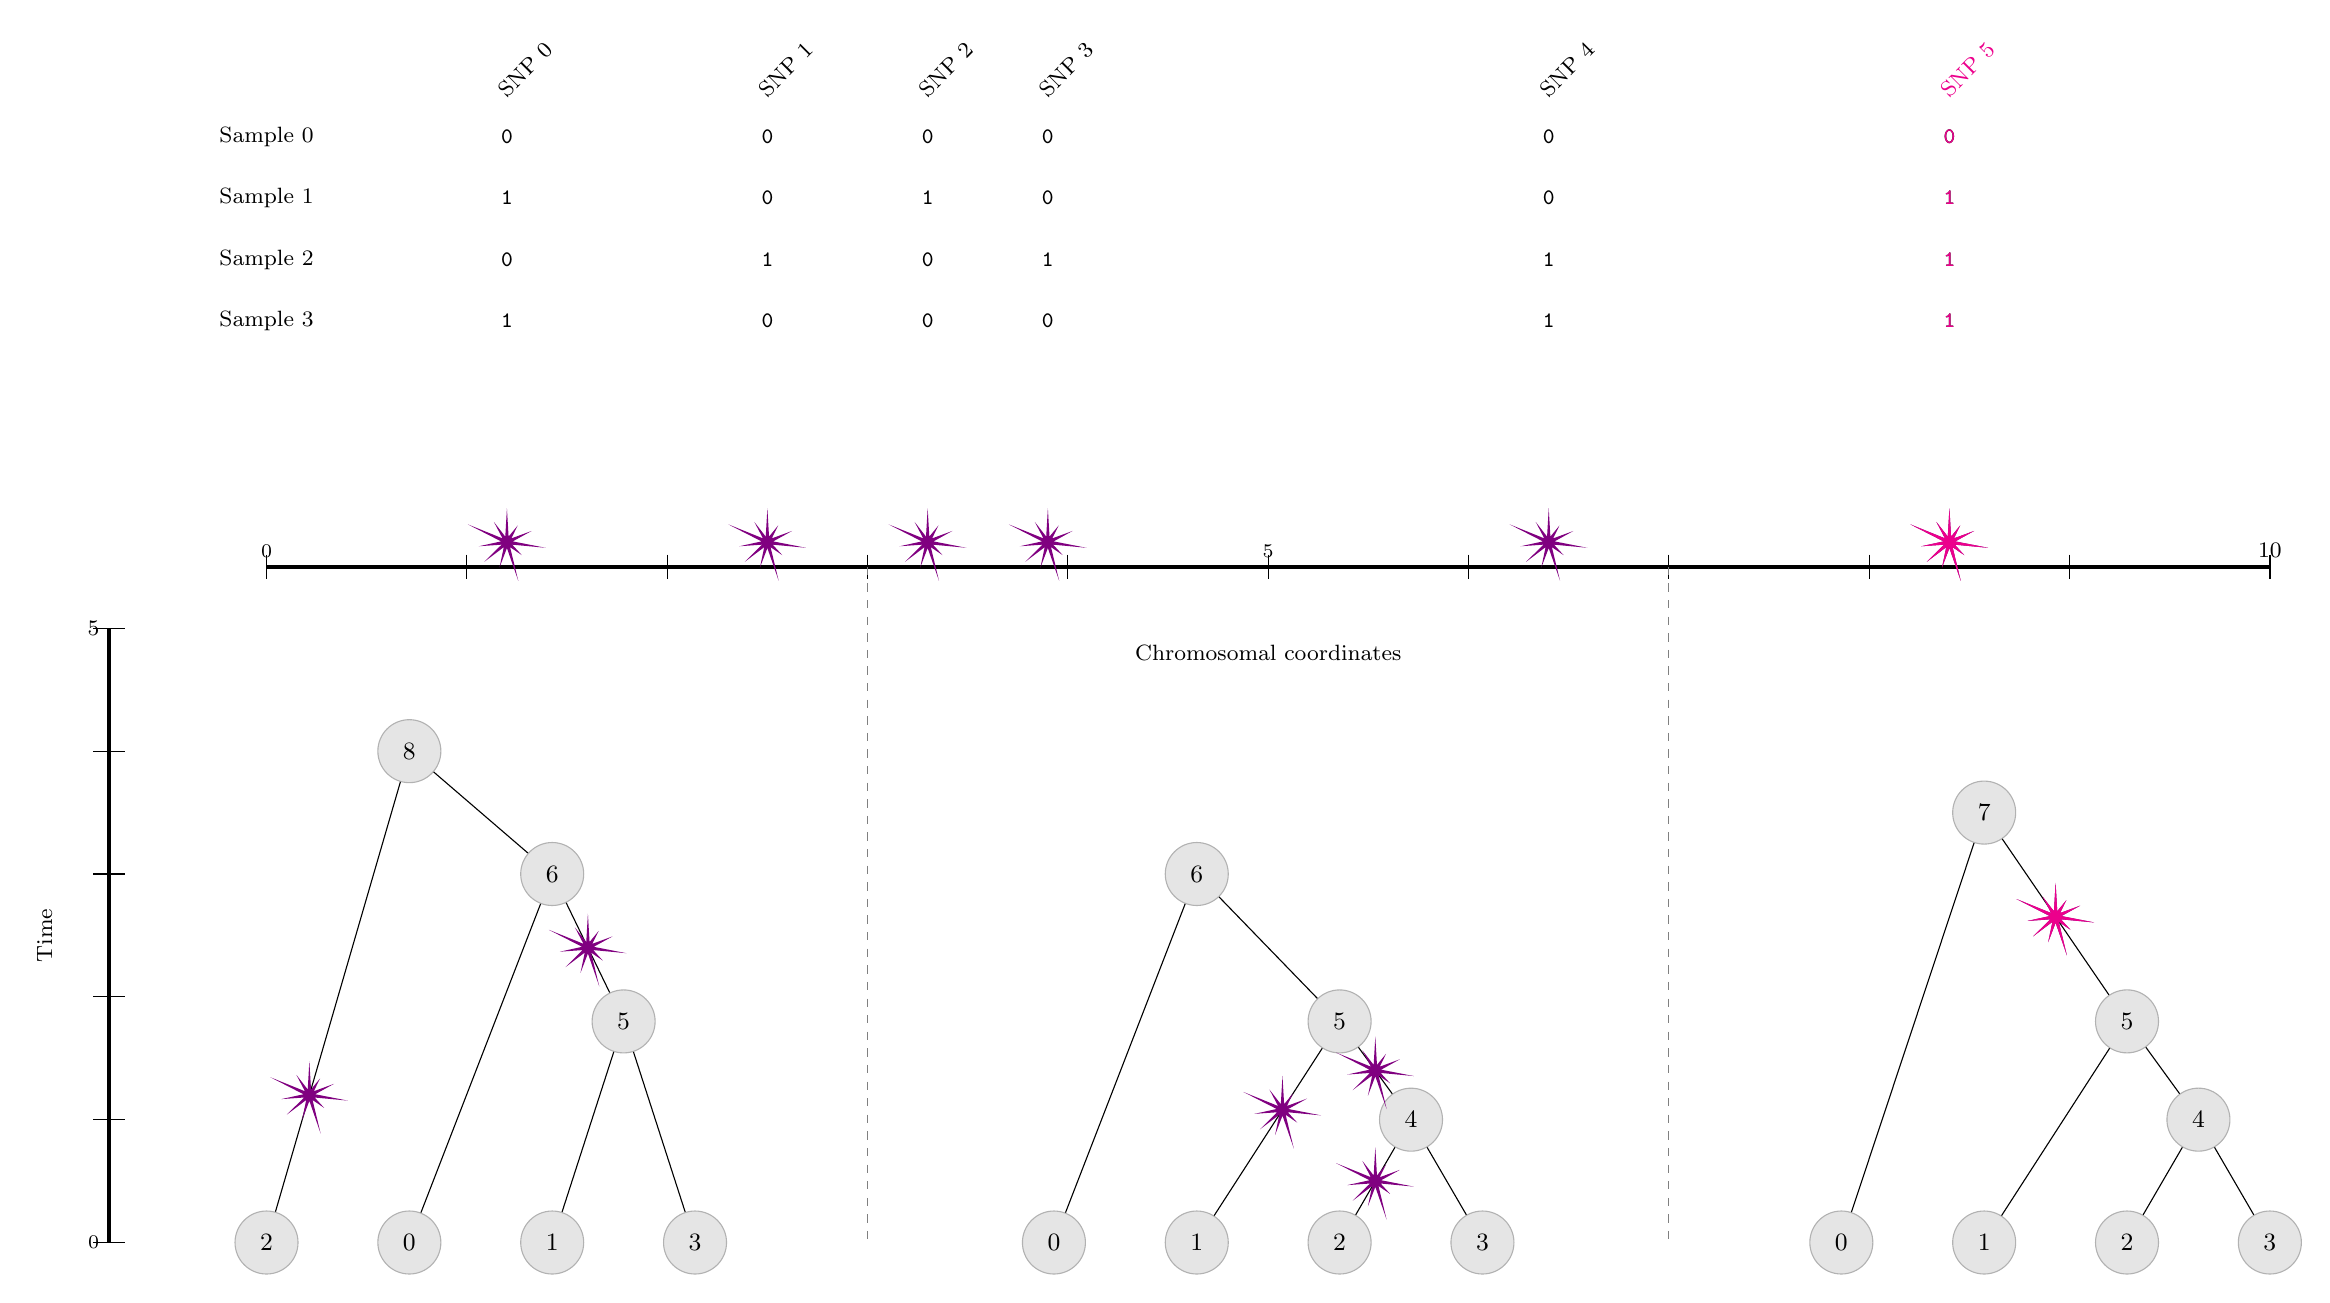
\begin{tikzpicture}[node distance=20mm and 10mm,yscale=1.56,xscale=2,font=\scriptsize]

\tikzset{greynode/.style={font=\small,node distance=4cm and 2cm,fill=black!10,draw=black!30,inner sep=0pt,minimum size=8mm,shape=circle},
mutations/.style={shape=starburst,fill=red!50!blue,inner sep=1.5pt,starburst points=11,starburst point height=.5cm}}

% Middle sample nodes
\node (s1) [greynode] {0};
\node (s2) [right=of s1,greynode] {1};
\node (s3) [right=of s2,greynode] {2};
\node (s4) [right=of s3,greynode] {3};

% Left sample nodes
\node (leftTree) at (-5, 0) {};
\node[greynode] (s3l) at ($(s1) + (leftTree)$) {2};
\node[greynode] (s1l) at ($(s2) + (leftTree)$) {0};
\node[greynode] (s2l) at ($(s3) + (leftTree)$) {1};
\node[greynode] (s4l) at ($(s4) + (leftTree)$) {3};

% Right sample nodes
\node (rightTree) at (5, 0) {};
\node [greynode] (s1r) at ($(s1) + (rightTree)$) {0};
\node [greynode] (s2r) at ($(s2) + (rightTree)$) {1};
\node [greynode] (s3r) at ($(s3) + (rightTree)$) {2};
\node [greynode] (s4r) at ($(s4) + (rightTree)$) {3};

% Non-sample nodes
\node [greynode] (s5) at ($0.5*(s3) + 0.5*(s4) + (0,1)$) {4};
\node [greynode] (s5r) at ($(s5) + (rightTree)$) {4};
\node [greynode] (s6) at ($(s3) + (0,1.8)$) {5};
\node [greynode] (s6r) at ($(s6) + (rightTree)$) {5};
\node [greynode] (s6l) at ($0.5*(s2l) + 0.5*(s4l) + (0,1.8)$) {5};
\node [greynode] (s7) at ($(s2) + (0,3)$) {6};
\node [greynode] (s7l) at ($(s2l) + (0,3)$) {6};
\node [greynode] (s8r) at ($(s2r) + (0,3.5)$) {7};
\node [greynode] (s9l) at ($(s1l) + (0,4)$) {8};

% Edges 
\draw (s6l) -- (s2l); \draw (s6l) -- (s4l); \draw (s7l) -- (s1l); \draw (s7l) -- (s6l); \draw (s3l) -- (s9l); \draw (s9l) -- (s7l); %tree 1
\draw (s5) -- (s3); \draw (s5) -- (s4); \draw (s6) -- (s2); \draw (s6) -- (s5); \draw (s7) -- (s1); \draw (s7) -- (s6); % tree 2
\draw (s5r) -- (s3r); \draw (s5r) -- (s4r); \draw (s6r) -- (s2r); \draw (s6r) -- (s5r); \draw (s8r) -- (s1r); \draw (s8r) -- (s6r); % tree 3

% Axes
\node (leftAx) at (-6,0) {};
\draw[very thick] (-6,0) -- +(0, 5);
\foreach \y in {0, 1, 2, 3, 4, 5} \draw ($(leftAx) + (-0.1, \y)$) -- ($(leftAx) + (0.1, \y)$); % tick marks
\draw[very thick] ($(s3l) + (0,5.5)$) -- ($(s4r) + (0,5.5)$);
\node (topAx) at (0,5.5) {};
\node (topLeft) at ($(s3l) + (0,5.5)$) {};
\node (genUnit) at ($0.1*(s4r) - 0.1*(s3l)$) {};
\foreach \x in {0, 1, 2, 3, 4, 5, 6, 7, 8, 9, 10} \draw ($(topLeft) + \x*(genUnit) + (0,0.1)$) -- +(0, -0.2); % tick marks
\node[anchor=east] at ($(leftAx)$) {0}; \node[anchor=east] at ($(leftAx) + (0,5)$) {\footnotesize 5};
\node[anchor=south] at ($(topLeft)$) {0}; \node[anchor=south] at ($(topLeft) + 5*(genUnit)$) {5}; \node[anchor=south] at ($(topLeft) + 10*(genUnit)$) {\footnotesize 10};

% Interval endpoints
\draw[thin,color=black!50,dashed] ($(topLeft) + 3*(genUnit)$) -- +(0, -5.5);
\draw[thin,color=black!50,dashed] ($(topLeft) + 7*(genUnit)$) -- +(0, -5.5);

% Mutations
\node[mutations] (m1) at ($(s3l)!0.3!(s9l)$) {};
\node[mutations] (m2) at ($(s6l)!0.5!(s7l)$) {};
\node[mutations] (m3) at ($(s2)!0.6!(s6)$) {};
\node[mutations] (m4) at ($(s3)!0.5!(s5)$) {};
\node[mutations] (m5) at ($(s5)!0.5!(s6)$) {};
\node[mutations] (m6) at ($(s6r)!0.5!(s8r)$) {};

% Axis titles
\node (topLabel) at ($(topLeft) + 5*(genUnit) + (0,-0.7)$) {\footnotesize Chromosomal coordinates};
\node[rotate=90,anchor=south] (leftLabel) at ($(leftAx) + (-0.3,2.5)$) {\footnotesize$\textrm{Time}$};

% Haplotypes
\node[font=\footnotesize] (hap1) at ($(topLeft) + (0,3.5)$) {\footnotesize$\textrm{Sample 0}$};
\node[font=\footnotesize] (hap2) at ($(topLeft) + (0,3)$) {\footnotesize$\textrm{Sample 1}$};
\node[font=\footnotesize] (hap3) at ($(topLeft) + (0,2.5)$) {\footnotesize$\textrm{Sample 2}$};
\node[font=\footnotesize] (hap4) at ($(topLeft) + (0,2)$) {\footnotesize$\textrm{Sample 3}$};

\foreach \x in {1.2, 2.5, 3.3, 3.9, 6.4, 8.4}  \node[mutations] () at ($(topLeft) + \x*(genUnit) + (0,.2)$) {};
\foreach \x in {1.2, 2.5, 3.3, 3.9, 6.4, 8.4} \node () at ($(hap1) + \x*(genUnit)$) {\footnotesize \texttt{0}};
\foreach \x in {2.5, 3.9, 6.4} \node () at ($(hap2) + \x*(genUnit)$) {\footnotesize \texttt{0}};
\foreach \x in {1.2, 3.3, 8.4} \node () at ($(hap2) + \x*(genUnit)$) {\footnotesize \texttt{1}};
\foreach \x in {1.2, 3.3} \node () at ($(hap3) + \x*(genUnit)$) {\footnotesize \texttt{0}};
\foreach \x in {2.5, 3.9, 6.4, 8.4} \node () at ($(hap3) + \x*(genUnit)$) {\footnotesize \texttt{1}};
\foreach \x in {2.5, 3.3, 3.9} \node () at ($(hap4) + \x*(genUnit)$) {\footnotesize \texttt{0}};
\foreach \x in {1.2, 6.4, 8.4} \node () at ($(hap4) + \x*(genUnit)$) {\footnotesize \texttt{1}};

% Magenta nodes and alleles
\node[color=magenta] at ($(hap1) + 8.4*(genUnit)$) {\footnotesize \texttt{0}};
\foreach \x in {2,3,4} \node[color=magenta] at ($(hap\x) + 8.4*(genUnit)$) {\footnotesize \texttt{1}};
\node[mutations,color=magenta] at  ($(topLeft) + 8.4*(genUnit) + (0,.2)$) {};
\node[mutations,color=magenta] at  (m6) {};

%\foreach \x in {1.2, 2.5, 3.3, 3.9, 6.4, 8.4} 
\node[rotate=45,anchor=south west]  at ($(hap1) + 1.2*(genUnit)+ (0,.2)$) {\footnotesize SNP 0};
\node[font=\footnotesize,rotate=45,anchor=south west]  at ($(hap1) + 2.5*(genUnit) + (0,.2)$) {\footnotesize SNP 1};
\node[font=\footnotesize,rotate=45,anchor=south west]  at ($(hap1) + 3.3*(genUnit)+ (0,.2)$) {\footnotesize SNP 2};
\node[font=\footnotesize,rotate=45,anchor=south west]  at ($(hap1) + 3.9*(genUnit)+ (0,.2)$) {\footnotesize SNP 3};
\node[font=\footnotesize,rotate=45,anchor=south west]  at ($(hap1) + 6.4*(genUnit)+ (0,.2)$) {\footnotesize SNP 4};
\node[font=\footnotesize,rotate=45,anchor=south west,color=magenta]  at ($(hap1) + 8.4*(genUnit)+ (0,.2)$) {\footnotesize {SNP 5}};

\end{tikzpicture}         
     }
     
     \block[bodyverticalshift=0cm]{3. Method outline}{} 
  \begin{subcolumns}
  \subcolumn{.48}
  \block{}{
  
\begin{tikzpicture}[node distance=2mm and 2mm,xscale=1,yscale=.9,font=\tiny]

\tikzset{greynode/.style={font=\footnotesize,node distance=1cm and 1 cm,fill=black!10,draw=black!30,inner sep=0pt,minimum size=3mm,shape=circle},
rednode/.style={font=\footnotesize,node distance=1cm and 1 cm,fill=red!30,draw=red!50,inner sep=0pt,minimum size=3mm,shape=circle},
bluenode/.style={font=\footnotesize,node distance=1cm and 1 cm,fill=blue!30,draw=blue!50,inner sep=0pt,minimum size=3mm,shape=circle},
purplenode/.style={font=\footnotesize,node distance=1cm and 1cm,fill=purple!30,draw=purple!50,inner sep=0pt,minimum size=3mm,shape=circle},
whitenode/.style={font=\footnotesize,node distance=1cm and 1cm,fill=white,draw=white,inner sep=0pt,minimum size=3.3mm,shape=circle}}

% Axis
\node (leftAx) at (-6,0) {};
\draw[very thick] (-6,0) -- +(0, 10);
\foreach \y in {0, 1, 2, 3, 4, 5, 6, 7, 8, 9, 10} \draw ($(leftAx) + (-0.1, \y)$) -- ($(leftAx) + (0.1, \y)$); % tick marks
\node[rotate=90,anchor=south] (leftLabel) at ($(leftAx) + (-0.3,5)$) {$\footnotesize\textrm{Time}$};

% Important times
\draw[gray,densely dashed] ($(leftAx) + (0,4)$) -- +(16, 0);

% Sample nodes
\node(s1) [purplenode] at (0,0) {};
\node (s2) [purplenode,right of=s1] {};
\node (s3) [purplenode,right of=s2] {};
\node (s4) [purplenode,right of=s3] {};

% Ancestral nodes
\node (pop1) at (-5, 4) {};
\node (pop2) at (5, 4) {};
\foreach \x in {1,2,3,4} \node[bluenode] (b\x) at ($(pop1) + (s\x)$) {};
\foreach \x in {1,2,3,4} \node[rednode] (r\x) at ($(pop2) + (s\x)$) {};

% Population labels
\node at ($0.5*(s2) + 0.5*(s3) + (0,-0.5)$) {$\tiny\textrm{Admixed population}$};
\node at ($(pop1) + 0.5*(s2) + 0.5*(s3) + (0,+0.5)$) {$\tiny\textrm{Blue ancestors}$};
\node at ($(pop2) + 0.5*(s2) + 0.5*(s3) + (0,+0.5)$) {$\tiny\textrm{Red ancestors}$};

% Cover the bottom bit
\foreach \x in {1,2,3,4} \node[whitenode] at (s\x) {};

% Time of admixture
\node[anchor=south,color=gray] at ($0.5*(b4) + 0.5*(r1)$) {{\tiny Start of admixture}};

% Step
\node at  ($0.5*(s2) + 0.5*(s3) + (0,9.5)$) {\small\gray{1. Initialise nodes from ancestral populations.}};

\end{tikzpicture} 

    
\begin{tikzpicture}[node distance=2mm and 2mm,xscale=1,yscale=.9,font=\tiny]

\tikzset{greynode/.style={font=\footnotesize,node distance=1cm and 1 cm,fill=black!10,draw=black!30,inner sep=0pt,minimum size=3mm,shape=circle},
rednode/.style={font=\footnotesize,node distance=1cm and 1 cm,fill=red!30,draw=red!50,inner sep=0pt,minimum size=3mm,shape=circle},
bluenode/.style={font=\footnotesize,node distance=1cm and 1 cm,fill=blue!30,draw=blue!50,inner sep=0pt,minimum size=3mm,shape=circle},
purplenode/.style={font=\footnotesize,node distance=1cm and 1cm,fill=purple!30,draw=purple!50,inner sep=0pt,minimum size=3mm,shape=circle},
whitenode/.style={font=\footnotesize,node distance=1cm and 1cm,fill=white,draw=white,inner sep=0pt,minimum size=3.3mm,shape=circle}}

% Axis
\node (leftAx) at (-6,0) {};
\draw[very thick] (-6,0) -- +(0, 10);
\foreach \y in {0, 1, 2, 3, 4, 5, 6, 7, 8, 9, 10} \draw ($(leftAx) + (-0.1, \y)$) -- ($(leftAx) + (0.1, \y)$); % tick marks
\node[rotate=90,anchor=south] (leftLabel) at ($(leftAx) + (-0.3,5)$) {\footnotesize$\textrm{Time}$};

% Important times
\draw[gray,densely dashed] ($(leftAx) + (0,4)$) -- +(14, 0);

% Sample nodes
\node[purplenode] (s1) at (0,0) {1};
\node (s2) [purplenode,right of=s1] {2};
\node (s3) [purplenode,right of=s2] {3};
\node (s4) [purplenode,right of=s3] {};
%
%% Other purple nodes
%
\foreach \x in {1,2,3,4} \foreach \y in {1,2,3} \node[purplenode] (u\x\y) at ($(s\x) + (0, \y)$) {};

% Ancestral nodes
\node (pop1) at (-5, 4) {};
\node (pop2) at (5, 4) {};
\foreach \x in {2,3} \node[bluenode] (b\x) at ($(pop1) + (s\x)$) {};
\foreach \x in {1,4} \node (b\x) at ($(pop1) + (s\x)$) {};
\foreach \x in {1,3,4} \node (r\x) at ($(pop2) + (s\x)$) {};
\node[rednode] (r2) at ($(pop2) + (s2)$) {};

% SLiM-simulated edges
\draw (s1) -- (u11) -- (u32) -- (u43) -- (r2);
\draw (s2) -- (u21) -- (u12) -- (u23) -- (b3);
\draw (s3) -- (u31) -- (u22) -- (u13) -- (b2);
\draw (s4) -- (u41) -- (u32) -- (u43);

% Population labels
%\node at ($0.5*(s1) + 0.5*(s3) + (0,-0.5)$) {$\tiny\textrm{Admixed samples}$};

% white nodes
\node[whitenode] at (u42){}; \node[whitenode] at (u33){};

% samples
%\draw[red,very thick] ($(s1.north)+(-.3,.3)$) -- ($(s3.north) + (.3,.3)$) -- ($(s3.south) + (.3,-.3)$) -- ($(s1.south)+(-.3,-.3)$)-- cycle;

% Time of admixture
\node[anchor=south,color=gray] at ($0.5*(b4) + 0.5*(r1)$) {{\tiny Start of admixture}};

% Population labels
\node at ($0.5*(s1) + 0.5*(s3) + (0,-0.5)$) {$\tiny\textrm{Admixed samples}$};

\end{tikzpicture} 

      
\begin{tikzpicture}[node distance=2mm and 2mm,xscale=1,yscale=.9,font=\tiny]

\tikzset{greynode/.style={font=\footnotesize,node distance=1cm and 1 cm,fill=black!10,draw=black!30,inner sep=0pt,minimum size=3mm,shape=circle},
rednode/.style={font=\footnotesize,node distance=1cm and 1 cm,fill=red!30,draw=red!50,inner sep=0pt,minimum size=3mm,shape=circle},
bluenode/.style={font=\footnotesize,node distance=1cm and 1 cm,fill=blue!30,draw=blue!50,inner sep=0pt,minimum size=3mm,shape=circle},
purplenode/.style={font=\footnotesize,node distance=1cm and 1cm,fill=purple!30,draw=purple!50,inner sep=0pt,minimum size=3mm,shape=circle},
whitenode/.style={font=\footnotesize,node distance=1cm and 1cm,fill=white,draw=white,inner sep=0pt,minimum size=3.3mm,shape=circle},
mutations/.style={shape=starburst,fill=red!50!blue,inner sep=0.8pt,starburst points=11,starburst point height=.2cm}}

% Axis
\node (leftAx) at (-6,0) {};
\draw[very thick] (-6,0) -- +(0, 10);
\foreach \y in {0, 1, 2, 3, 4, 5, 6, 7, 8, 9, 10} \draw ($(leftAx) + (-0.1, \y)$) -- ($(leftAx) + (0.1, \y)$); % tick marks
\node[rotate=90,anchor=south] (leftLabel) at ($(leftAx) + (-0.3,5)$) {$\footnotesize\textrm{Time}$};

% Important times
\draw[gray,densely dashed] ($(leftAx) + (0,4)$) -- +(14, 0);

% Sample nodes
\node[purplenode] (s1) at (0,0) {1};
\node (s2) [purplenode,right of=s1] {2};
\node (s3) [purplenode,right of=s2] {3};
\node (s4) [purplenode,right of=s3] {};
%
%% Other purple nodes
%
\foreach \x in {1,2,3,4} \foreach \y in {1,2,3} \node[purplenode] (u\x\y) at ($(s\x) + (0, \y)$) {};

% Ancestral nodes
\node (pop1) at (-5, 4) {};
\node (pop2) at (5, 4) {};
\foreach \x in {2,3} \node[bluenode] (b\x) at ($(pop1) + (s\x)$) {};
\foreach \x in {1,4} \node (b\x) at ($(pop1) + (s\x)$) {};
\foreach \x in {1,3,4} \node (r\x) at ($(pop2) + (s\x)$) {};
\node[rednode] (r2) at ($(pop2) + (s2)$) {};

% white nodes
\node[whitenode] at (u42){}; \node[whitenode] at (u33){};
\node[whitenode] at (s4){}; \node[whitenode] at (u41){};
\foreach \x in {1,2,3,4} \foreach \y in {1,2,3} \node[whitenode] (u\x\y) at ($(s\x) + (0, \y)$) {};

% samples
%\draw[red,very thick] ($(s1.north)+(-.3,.3)$) -- ($(s3.north) + (.3,.3)$) -- ($(s3.south) + (.3,-.3)$) -- ($(s1.south)+(-.3,-.3)$)-- cycle;

% Time of admixture
\node[anchor=south,color=gray] at ($0.5*(b4) + 0.5*(r1)$) {{\tiny Start of admixture}};

% SLiM-simulated edges
\draw (s1) -- (u11.center) -- (u32.center) -- (u43.center) -- (r2);
\draw (s2) -- (u21.center) -- (u12.center) -- (u23.center) -- (b3);
\draw (s3) -- (u31.center) -- (u22.center) -- (u13.center) -- (b2);
\draw (u32.center) -- (u43.center);

% Mutations
\node[mutations] at ($(u11)!.5!(u32)$) {};
\node[mutations] at ($(u13)!.7!(u22)$) {};

% msprime nodes
\node[bluenode] (b5) at ($0.5*(b2)+0.5*(b3)+(0,1.8)$) {}; 
\node[greynode] (g1) at ($0.5*(b5)+0.5*(r2)+(0,3.6)$) {};

% msprime edges
\draw (b2) -- (b5) -- (b3); \draw (b5) -- (g1) -- (r2);

% simulation label
\draw[very thick,->,magenta] ($(b1) + (0,0.1)$) -- +(0,5.9);
\node[rotate=90,anchor=south,magenta] (msprime) at ($(b1) + (0,3)$) {$\texttt{msprime}$};

% Time of admixture
\node[anchor=south,color=gray] at ($0.5*(b4) + 0.5*(r1)$) {{\tiny Start of admixture}};

\end{tikzpicture} 

  }
  \subcolumn{.48}
   \block{}{
  
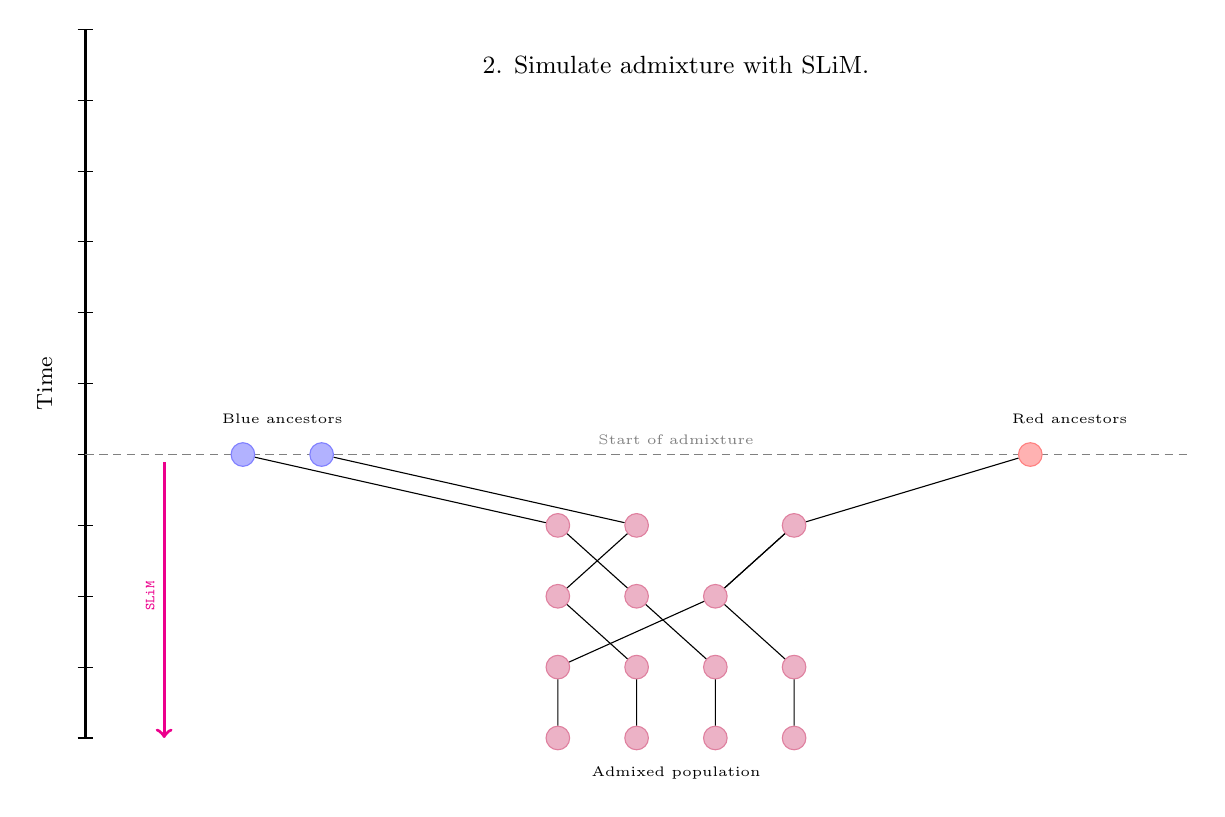
\begin{tikzpicture}[node distance=2mm and 2mm,xscale=1,yscale=.9,font=\tiny]

\tikzset{greynode/.style={font=\footnotesize,node distance=1cm and 1 cm,fill=black!10,draw=black!30,inner sep=0pt,minimum size=3mm,shape=circle},
rednode/.style={font=\footnotesize,node distance=1cm and 1 cm,fill=red!30,draw=red!50,inner sep=0pt,minimum size=3mm,shape=circle},
bluenode/.style={font=\footnotesize,node distance=1cm and 1 cm,fill=blue!30,draw=blue!50,inner sep=0pt,minimum size=3mm,shape=circle},
purplenode/.style={font=\footnotesize,node distance=1cm and 1cm,fill=purple!30,draw=purple!50,inner sep=0pt,minimum size=3mm,shape=circle},
whitenode/.style={font=\footnotesize,node distance=1cm and 1cm,fill=white,draw=white,inner sep=0pt,minimum size=3.3mm,shape=circle}}

% Axis
\node (leftAx) at (-6,0) {};
\draw[very thick] (-6,0) -- +(0, 10);
\foreach \y in {0, 1, 2, 3, 4, 5, 6, 7, 8, 9, 10} \draw ($(leftAx) + (-0.1, \y)$) -- ($(leftAx) + (0.1, \y)$); % tick marks
\node[rotate=90,anchor=south] (leftLabel) at ($(leftAx) + (-0.3,5)$) {\footnotesize$\textrm{Time}$};

% Important times
\draw[gray,densely dashed] ($(leftAx) + (0,4)$) -- +(14, 0);

% Sample nodes
\node[purplenode] (s1) at (0,0) {};
\node (s2) [purplenode,right of=s1] {};
\node (s3) [purplenode,right of=s2] {};
\node (s4) [purplenode,right of=s3] {};
%
%% Other purple nodes
%
\foreach \x in {1,2,3,4} \foreach \y in {1,2,3} \node[purplenode] (u\x\y) at ($(s\x) + (0, \y)$) {};

% Ancestral nodes
\node (pop1) at (-5, 4) {};
\node (pop2) at (5, 4) {};
\foreach \x in {2,3} \node[bluenode] (b\x) at ($(pop1) + (s\x)$) {};
\foreach \x in {1,4} \node (b\x) at ($(pop1) + (s\x)$) {};
\foreach \x in {1,3,4} \node (r\x) at ($(pop2) + (s\x)$) {};
\node[rednode] (r2) at ($(pop2) + (s2)$) {};

% SLiM-simulated edges
\draw (s1) -- (u11) -- (u32) -- (u43) -- (r2);
\draw (s2) -- (u21) -- (u12) -- (u23) -- (b3);
\draw (s3) -- (u31) -- (u22) -- (u13) -- (b2);
\draw (s4) -- (u41) -- (u32) -- (u43);

% Population labels
\node at ($0.5*(s2) + 0.5*(s3) + (0,-0.5)$) {$\tiny\textrm{Admixed population}$};
\node at ($(pop1) + 0.5*(s2) + 0.5*(s3) + (0,+0.5)$) {$\tiny\textrm{Blue ancestors}$};
\node at ($(pop2) + 0.5*(s2) + 0.5*(s3) + (0,+0.5)$) {$\tiny\textrm{Red ancestors}$};

% white nodes
\node[whitenode] at (u42){}; \node[whitenode] at (u33){};

% simulation label
\draw[very thick,<-,magenta] ($(s1) + (-5,0)$) -- +(0,3.9);
\node[rotate=90,anchor=south,magenta] (SLiM) at ($(s1) + (-5,0) + (0,2)$) {$\texttt{SLiM}$};

% Time of admixture
\node[anchor=south,color=gray] at ($0.5*(b4) + 0.5*(r1)$) {{\tiny Start of admixture}};

% Step
\node at  ($0.5*(s2) + 0.5*(s3) + (0,9.5)$) {\small\gray{2. Simulate admixture with SLiM.}};

\end{tikzpicture} 

    
\begin{tikzpicture}[node distance=2mm and 2mm,xscale=1,yscale=.9,font=\tiny]

\tikzset{greynode/.style={font=\footnotesize,node distance=1cm and 1 cm,fill=black!10,draw=black!30,inner sep=0pt,minimum size=3mm,shape=circle},
rednode/.style={font=\footnotesize,node distance=1cm and 1 cm,fill=red!30,draw=red!50,inner sep=0pt,minimum size=3mm,shape=circle},
bluenode/.style={font=\footnotesize,node distance=1cm and 1 cm,fill=blue!30,draw=blue!50,inner sep=0pt,minimum size=3mm,shape=circle},
purplenode/.style={font=\footnotesize,node distance=1cm and 1cm,fill=purple!30,draw=purple!50,inner sep=0pt,minimum size=3mm,shape=circle},
whitenode/.style={font=\footnotesize,node distance=1cm and 1cm,fill=white,draw=white,inner sep=0pt,minimum size=3.3mm,shape=circle}}

% Axis
\node (leftAx) at (-6,0) {};
\draw[very thick] (-6,0) -- +(0, 10);
\foreach \y in {0, 1, 2, 3, 4, 5, 6, 7, 8, 9, 10} \draw ($(leftAx) + (-0.1, \y)$) -- ($(leftAx) + (0.1, \y)$); % tick marks
\node[rotate=90,anchor=south] (leftLabel) at ($(leftAx) + (-0.3,5)$) {$\footnotesize\textrm{Time}$};

% Important times
\draw[gray,densely dashed] ($(leftAx) + (0,4)$) -- +(14, 0);

% Sample nodes
\node[purplenode] (s1) at (0,0) {1};
\node (s2) [purplenode,right of=s1] {2};
\node (s3) [purplenode,right of=s2] {3};
\node (s4) [purplenode,right of=s3] {};
%
%% Other purple nodes
%
\foreach \x in {1,2,3,4} \foreach \y in {1,2,3} \node[purplenode] (u\x\y) at ($(s\x) + (0, \y)$) {};

% Ancestral nodes
\node (pop1) at (-5, 4) {};
\node (pop2) at (5, 4) {};
\foreach \x in {2,3} \node[bluenode] (b\x) at ($(pop1) + (s\x)$) {};
\foreach \x in {1,4} \node (b\x) at ($(pop1) + (s\x)$) {};
\foreach \x in {1,3,4} \node (r\x) at ($(pop2) + (s\x)$) {};
\node[rednode] (r2) at ($(pop2) + (s2)$) {};

% Population labels
\node at ($0.5*(s1) + 0.5*(s3) + (0,-0.5)$) {$\tiny\textrm{Admixed samples}$};

% Population labels
%\node at ($0.5*(s1) + 0.5*(s3) + (0,-0.5)$) {$\tiny\textrm{Admixed samples}$};

% white nodes
\node[whitenode] at (u42){}; \node[whitenode] at (u33){};
\node[whitenode] at (s4){}; \node[whitenode] at (u41){};
\foreach \x in {1,2,3,4} \foreach \y in {1,2,3} \node[whitenode] (u\x\y) at ($(s\x) + (0, \y)$) {};

% samples
%\draw[red,very thick] ($(s1.north)+(-.3,.3)$) -- ($(s3.north) + (.3,.3)$) -- ($(s3.south) + (.3,-.3)$) -- ($(s1.south)+(-.3,-.3)$)-- cycle;

% Time of admixture
\node[anchor=south,color=gray] at ($0.5*(b4) + 0.5*(r1)$) {{\tiny Start of admixture}};

% SLiM-simulated edges
\draw (s1) -- (u11.center) -- (u32.center) -- (u43.center) -- (r2);
\draw (s2) -- (u21.center) -- (u12.center) -- (u23.center) -- (b3);
\draw (s3) -- (u31.center) -- (u22.center) -- (u13.center) -- (b2);
\draw (u32.center) -- (u43.center);

% Step
\node at  ($0.5*(s2) + 0.5*(s3) + (0,9.5)$) {\small\gray{4. Simplify tree sequence.}};

\end{tikzpicture} 

      
\begin{tikzpicture}[node distance=2mm and 2mm,xscale=1,yscale=.9,font=\tiny]

\tikzset{greynode/.style={font=\footnotesize,node distance=1cm and 1 cm,fill=black!10,draw=black!30,inner sep=0pt,minimum size=3mm,shape=circle},
rednode/.style={font=\footnotesize,node distance=1cm and 1 cm,fill=red!30,draw=red!50,inner sep=0pt,minimum size=3mm,shape=circle},
bluenode/.style={font=\footnotesize,node distance=1cm and 1 cm,fill=blue!30,draw=blue!50,inner sep=0pt,minimum size=3mm,shape=circle},
purplenode/.style={font=\footnotesize,node distance=1cm and 1cm,fill=purple!30,draw=purple!50,inner sep=0pt,minimum size=3mm,shape=circle},
whitenode/.style={font=\footnotesize,node distance=1cm and 1cm,fill=white,draw=white,inner sep=0pt,minimum size=3.3mm,shape=circle},
mutations/.style={shape=starburst,fill=red!50!blue,inner sep=0.8pt,starburst points=11,starburst point height=.2cm}}

% Axis
\node (leftAx) at (-6,0) {};
\draw[very thick] (-6,0) -- +(0, 10);
\foreach \y in {0, 1, 2, 3, 4, 5, 6, 7, 8, 9, 10} \draw ($(leftAx) + (-0.1, \y)$) -- ($(leftAx) + (0.1, \y)$); % tick marks
\node[rotate=90,anchor=south] (leftLabel) at ($(leftAx) + (-0.3,5)$) {$\footnotesize\textrm{Time}$};

% Important times
\draw[gray,densely dashed] ($(leftAx) + (0,4)$) -- +(14, 0);

% Sample nodes
\node[purplenode] (s1) at (0,0) {1};
\node (s2) [purplenode,right of=s1] {2};
\node (s3) [purplenode,right of=s2] {3};
\node (s4) [purplenode,right of=s3] {};
%
%% Other purple nodes
%
\foreach \x in {1,2,3,4} \foreach \y in {1,2,3} \node[purplenode] (u\x\y) at ($(s\x) + (0, \y)$) {};

% Ancestral nodes
\node (pop1) at (-5, 4) {};
\node (pop2) at (5, 4) {};
\foreach \x in {2,3} \node[bluenode] (b\x) at ($(pop1) + (s\x)$) {};
\foreach \x in {1,4} \node (b\x) at ($(pop1) + (s\x)$) {};
\foreach \x in {1,3,4} \node (r\x) at ($(pop2) + (s\x)$) {};
\node[rednode] (r2) at ($(pop2) + (s2)$) {};

% white nodes
\node[whitenode] at (u42){}; \node[whitenode] at (u33){};
\node[whitenode] at (s4){}; \node[whitenode] at (u41){};
\foreach \x in {1,2,3,4} \foreach \y in {1,2,3} \node[whitenode] (u\x\y) at ($(s\x) + (0, \y)$) {};

% samples
%\draw[red,very thick] ($(s1.north)+(-.3,.3)$) -- ($(s3.north) + (.3,.3)$) -- ($(s3.south) + (.3,-.3)$) -- ($(s1.south)+(-.3,-.3)$)-- cycle;

% Time of admixture
\node[anchor=south,color=gray] at ($0.5*(b4) + 0.5*(r1)$) {{\tiny Start of admixture}};

% SLiM-simulated edges
\draw (s1) -- (u11.center) -- (u32.center) -- (u43.center) -- (r2);
\draw (s2) -- (u21.center) -- (u12.center) -- (u23.center) -- (b3);
\draw (s3) -- (u31.center) -- (u22.center) -- (u13.center) -- (b2);
\draw (u32.center) -- (u43.center);

% msprime nodes
\node[bluenode] (b5) at ($0.5*(b2)+0.5*(b3)+(0,1.8)$) {}; 
\node[greynode] (g1) at ($0.5*(b5)+0.5*(r2)+(0,3.6)$) {};

% msprime edges
\draw (b2) -- (b5) -- (b3); \draw (b5) -- (g1) -- (r2);

% simulation label
\draw[very thick,->,magenta] ($(b1) + (0,0.1)$) -- +(0,5.9);
\node[rotate=90,anchor=south,magenta] (msprime) at ($(b1) + (0,3)$) {$\texttt{msprime}$};

% Time of admixture
\node[anchor=south,color=gray] at ($0.5*(b4) + 0.5*(r1)$) {{\tiny Start of admixture}};

% Mutations
\node[mutations] at ($(u11)!.5!(u32)$) {};
\node[mutations] at ($(u13)!.7!(u22)$) {};
\node[mutations] at ($(b5)!.6!(b3)$) {};
\node[mutations] at ($(r2)!.7!(g1)$) {};

\end{tikzpicture} 

  }
  \end{subcolumns}
     


     \column{.5}
     %%% BLOCK 2
         \block[bodyverticalshift=0cm,titleoffsety=-12cm,bodyoffsety=-12cm]{2. Local ancestry in tree sequences}{}  
          \begin{subcolumns}       
         \subcolumn{.45}
          \block{}{
          This is real hard. See why below:
          
          \begin{center}
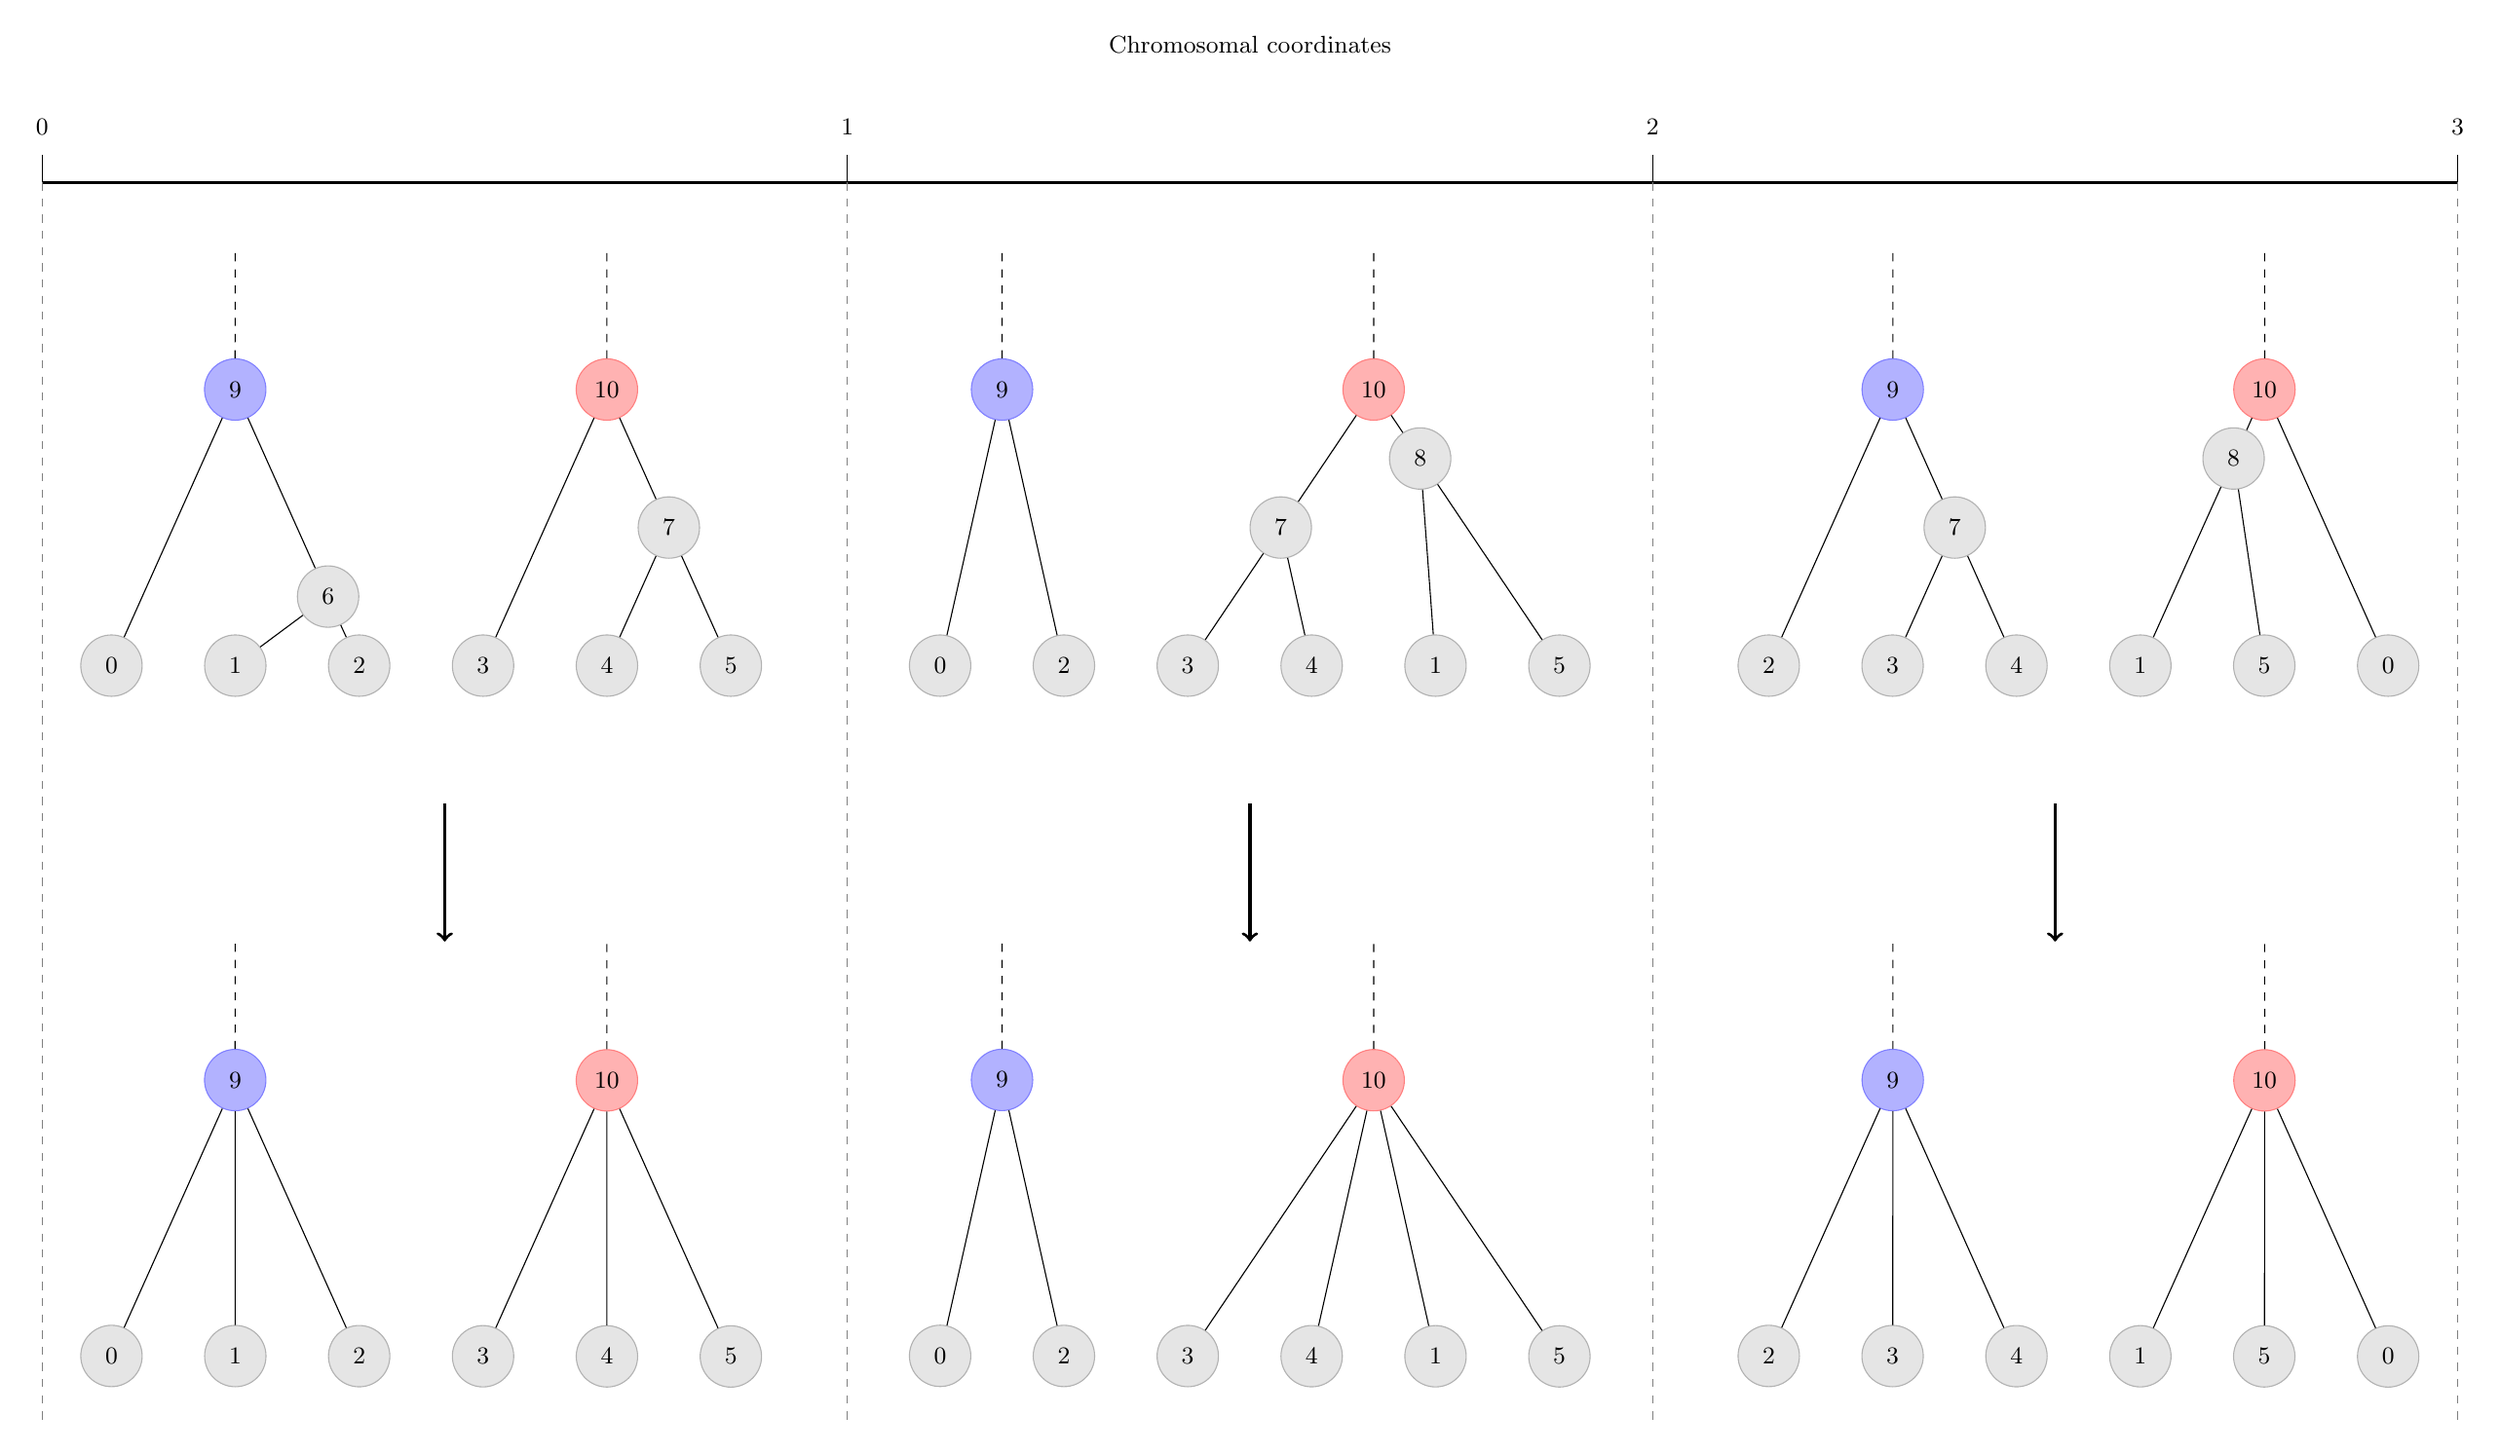
\begin{tikzpicture}[node distance=8mm and 8mm,xscale=1.8,yscale=1.8]

\tikzset{greynode/.style={font=\small,node distance=.5cm and .5 cm,fill=black!10,draw=black!30,inner sep=0pt,minimum size=8mm,shape=circle},
bluenode/.style={font=\small,node distance=.5cm and .5cm,fill=blue!30,draw=blue!50,inner sep=0pt,minimum size=8mm,shape=circle},
rednode/.style={font=\small,node distance=.5cm and .5cm,fill=red!30,draw=red!50,inner sep=0pt,minimum size=8mm,shape=circle}}

% Middle sample nodes
\node (s0) [greynode] {0};
\node (s2) [right=of s0,greynode] {2};
\node (s3) [right=of s2,greynode] {3};
\node (s4) [right=of s3,greynode] {4};
\node (s1) [right=of s4,greynode] {1};
\node (s5) [right=of s1,greynode] {5};

% Left sample nodes
\node (leftTree) at (-6, 0) {};
\node[greynode] (s0l) at ($(s0) + (leftTree)$) {0};
\node[greynode] (s1l) at ($(s2) + (leftTree)$) {1};
\node[greynode] (s2l) at ($(s3) + (leftTree)$) {2};
\node[greynode] (s3l) at ($(s4) + (leftTree)$) {3};
\node[greynode] (s4l) at ($(s1) + (leftTree)$) {4};
\node[greynode] (s5l) at ($(s5) + (leftTree)$) {5};

% Right sample nodes
\node (rightTree) at (6, 0) {};
\node [greynode] (s2r) at ($(s0) + (rightTree)$) {2};
\node [greynode] (s3r) at ($(s2) + (rightTree)$) {3};
\node [greynode] (s4r) at ($(s3) + (rightTree)$) {4};
\node [greynode] (s1r) at ($(s4) + (rightTree)$) {1};
\node [greynode] (s5r) at ($(s1) + (rightTree)$) {5};
\node [greynode] (s0r) at ($(s5) + (rightTree)$) {0};

% Ancestral nodes
\node (anc) at (0,2) {};
\node[bluenode] (s9) at ($0.5*(s0) + 0.5*(s2) + (anc)$) {9};
\node[bluenode] (s9l) at ($0.5*(s0l) + 0.5*(s2l) + (anc)$) {9};
\node[bluenode] (s9r) at ($0.5*(s2r) + 0.5*(s4r) + (anc)$) {9};
\node[rednode] (s10) at ($0.5*(s3)+0.5*(s5) + (anc)$) {10};
\node[rednode] (s10l) at ($0.5*(s3l)+0.5*(s5l) + (anc)$) {10};
\node[rednode] (s10r) at ($0.5*(s1r)+0.5*(s0r) + (anc)$) {10};

% Internal nodes
\node[greynode] (s6l) at ($(s2l)!0.25!(s9l)$) {6};
\node[greynode] (s7) at ($(s3)!.5!(s10)$) {7};
\node[greynode] (s7l) at ($(s5l)!.5!(s10l)$) {7};
\node[greynode] (s7r) at ($(s4r)!.5!(s9r)$) {7};
\node[greynode] (s8) at ($(s5)!.75!(s10)$) {8};
\node[greynode] (s8r) at ($(s1r)!.75!(s10r)$) {8};

% Edges
\draw (s0) -- (s9) -- (s2); \draw (s3) -- (s7) -- (s10) -- (s8) -- (s5); \draw (s4) -- (s7); \draw (s1) -- (s8); % middle tree
\draw (s0l) -- (s9l) -- (s6l) -- (s2l); \draw (s1l) -- (s6l); \draw ( s3l) -- (s10l) -- (s7l) -- (s5l); \draw (s4l) -- (s7l); % left tree
\draw (s2r) -- (s9r) -- (s7r) -- (s4r); \draw (s3r) -- (s7r); \draw (s1r) -- (s8r) -- (s10r) -- (s0r); \draw (s5r) -- (s8r); % right tree
\draw[dashed] (s9) -- +(0,1); \draw[dashed] (s9l) -- +(0,1); \draw[dashed] (s9r) -- +(0,1);
\draw[dashed] (s10) -- +(0,1); \draw[dashed] (s10l) -- +(0,1); \draw[dashed] (s10r) -- +(0,1);

% Axes
\node (topAx) at (0,3.5) {};
\node (topLeft) at ($(s0l) + (topAx) + (-0.5, 0)$) {};
\node (topRight) at ($(s0r) + (topAx) + (0.5,0)$) {};
\draw[very thick] (topLeft.center) -- (topRight.center);
\node (genunit) at ($0.3333*(topRight) - 0.3333*(topLeft)$) {};
\foreach \x in {0,1,2,3} \draw ($(topLeft) + \x*(genunit)$) -- +(0,.2);
\foreach \x in {0,1,2,3} \node at ($(topLeft) + \x*(genunit) + (0,.4)$) {\small\x};

% Interval endpoints
\foreach \x in {0,1,2,3} \draw[thin,color=black!50,dashed] ($(topLeft) + \x*(genunit)$) -- +(0, -9);
%\draw[thin,color=black!50,dashed] ($(topLeft) + 7*(genUnit)$) -- +(0, -5.5);

% Axis titles
\node (topLabel) at ($(topLeft) + 1.5*(genunit) + (0,1)$) {\small$\textrm{Chromosomal coordinates}$};

%%%%%
\node (after) at (0, -5) {};

% Middle sample nodes
\node[greynode] (s0) at (after) {0};
\node (s2) [right=of s0,greynode] {2};
\node (s3) [right=of s2,greynode] {3};
\node (s4) [right=of s3,greynode] {4};
\node (s1) [right=of s4,greynode] {1};
\node (s5) [right=of s1,greynode] {5};

% Left sample nodes
\node (leftTree) at (-6, 0) {};
\node[greynode] (s0l) at ($(s0) + (leftTree)$) {0};
\node[greynode] (s1l) at ($(s2) + (leftTree)$) {1};
\node[greynode] (s2l) at ($(s3) + (leftTree)$) {2};
\node[greynode] (s3l) at ($(s4) + (leftTree)$) {3};
\node[greynode] (s4l) at ($(s1) + (leftTree)$) {4};
\node[greynode] (s5l) at ($(s5) + (leftTree)$) {5};

% Right sample nodes
\node (rightTree) at (6, 0) {};
\node [greynode] (s2r) at ($(s0) + (rightTree)$) {2};
\node [greynode] (s3r) at ($(s2) + (rightTree)$) {3};
\node [greynode] (s4r) at ($(s3) + (rightTree)$) {4};
\node [greynode] (s1r) at ($(s4) + (rightTree)$) {1};
\node [greynode] (s5r) at ($(s1) + (rightTree)$) {5};
\node [greynode] (s0r) at ($(s5) + (rightTree)$) {0};

% Ancestral nodes
\node (anc) at (0,2) {};
\node[bluenode] (s9) at ($0.5*(s0) + 0.5*(s2) + (anc)$) {9};
\node[bluenode] (s9l) at ($0.5*(s0l) + 0.5*(s2l) + (anc)$) {9};
\node[bluenode] (s9r) at ($0.5*(s2r) + 0.5*(s4r) + (anc)$) {9};
\node[rednode] (s10) at ($0.5*(s3)+0.5*(s5) + (anc)$) {10};
\node[rednode] (s10l) at ($0.5*(s3l)+0.5*(s5l) + (anc)$) {10};
\node[rednode] (s10r) at ($0.5*(s1r)+0.5*(s0r) + (anc)$) {10};

%% Axes
%\node (topAx) at (0,3.5) {};
%\node (topLeft) at ($(s0l) + (topAx) + (-0.5, 0)$) {};
%\node (topRight) at ($(s0r) + (topAx) + (0.5,0)$) {};
%\draw[very thick] (topLeft.center) -- (topRight.center);
%\node (genunit) at ($0.3333*(topRight) - 0.3333*(topLeft)$) {};
%\foreach \x in {0,1,2,3} \draw ($(topLeft) + \x*(genunit)$) -- +(0,.2);
%\foreach \x in {0,1,2,3} \node at ($(topLeft) + \x*(genunit) + (0,.4)$) {\x};

% Edges
\draw (s0) -- (s9) -- (s2); \draw (s3) -- (s10) -- (s4); \draw (s1) -- (s10) --  (s5); % middle tree
\draw (s0l) -- (s9l) -- (s2l); \draw (s1l) -- (s9l); \draw (s3l) -- (s10l) -- (s5l); \draw (s4l) -- (s10l); % left tree
\draw (s2r) -- (s9r) -- (s3r); \draw (s4r) -- (s9r); \draw (s1r) -- (s10r) -- (s5r); \draw (s0r) -- (s10r);

\draw[dashed] (s9) -- +(0,1); \draw[dashed] (s9l) -- +(0,1); \draw[dashed] (s9r) -- +(0,1);
\draw[dashed] (s10) -- +(0,1); \draw[dashed] (s10l) -- +(0,1); \draw[dashed] (s10r) -- +(0,1);

% Interval endpoints
\foreach \x in {0,1,2,3} \draw[thin,color=black!50,dashed] ($(topLeft) + \x*(genunit)$) -- +(0, -4);
%\draw[thin,color=black!50,dashed] ($(topLeft) + 7*(genUnit)$) -- +(0, -5.5);

%% Axis titles
%\node (topLabel) at ($(topLeft) + 1.5*(genunit) + (0,1)$) {$\textrm{Chromosomal coordinates}$};

%% Arrows
\foreach \x in {0, 1, 2} \draw[<-,very thick] ($(topLeft) + \x*(genunit) + 0.5*(genunit) + (0,-5.5)$) -- +(0, 1);

\end{tikzpicture}
\end{center} 

          }           
         \end{subcolumns}
         

 
         
\vspace{20cm}

%         \begin{subcolumns}
%             \subcolumn{.45}
             \block{4. Method performance}{If you want to have an additional subdivision of columns inside a column, you may use the\\ \texttt{\bs subcolumns} environment inside of a column environment.  The functionality is similar to that of columns, but now the widths are relative to the width of the current column.}

     \end{columns}
     
 \block[titleoffsety=-20cm,bodyoffsety=-20cm]{5. Acknowledgements and references}{
blah 	
 }
           

 \end{document}




\endinput
%%
%% End of file `tikzposter-example.tex'.
